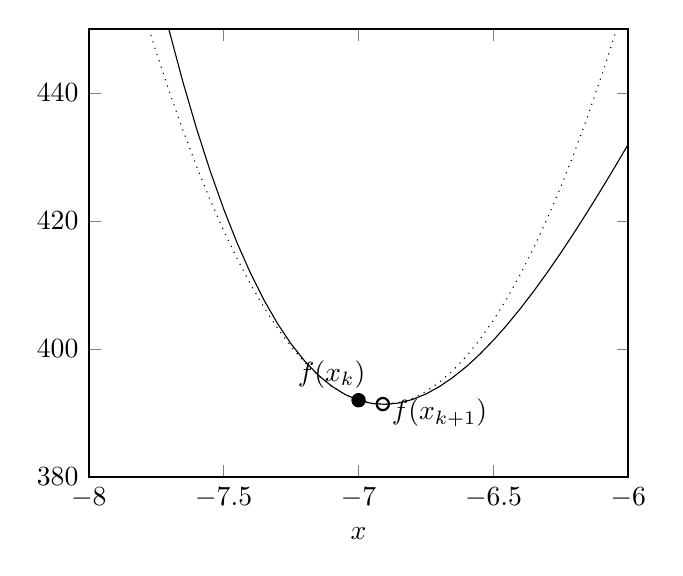
\begin{tikzpicture}
  \begin{axis}[
      xlabel={$x$},
      samples=41,
      thick,
      domain=-8:-6,
      xmin=-8,
      xmax=-6,
      ymin=380,
      ymax=450,
    ]
    \addplot+[
      mark=none,
      mark color=black,
      color=black,
      thin
    ] {2 * x^4 + 30 * x^3 + 120 * x^2 };
    \addplot+[
      mark=none,
      mark color=black,
      color=black,
      thin,
      dotted
    ] {392 + (x + 7) * (-14) + 0.5 * (x + 7)  *156 * (x + 7)};
    \node at (-7.1, 396) {$f(x_k)$};
    \node at (-6.7, 390) {$f(x_{k+1})$};
    \draw (-7, 392) circle[radius=2.2pt];
    \fill (-7, 392) circle[radius=2.2pt];
    \draw (-6.91, 391.4) circle[radius=2.2pt];
\end{axis}
\end{tikzpicture}
